\documentclass[a4paper]{article}
\usepackage{amsmath}
\usepackage{amssymb}
\usepackage{geometry}
\usepackage{enumerate}
\usepackage{float}%稳定图片位置
\usepackage{graphicx}%画图
\usepackage{wrapfig}
\usepackage{indentfirst}%缩进
\usepackage{enumerate}%加序号
\usepackage{multirow}%合并行
\usepackage{subfigure}
\usepackage{graphicx}
\usepackage{hyperref}
\usepackage[bottom]{footmisc}
\usepackage{listings}
\usepackage{xcolor}
\usepackage{pdfpages}
\title{\Large \textbf{VP390 Bonus Question Set 1}\\
\author{\textbf{Pan, Chongdan ID:516370910121}\\
}
}
\begin{document}
\maketitle
    For the stationery equation $-\frac{\hbar^2}{2m}\frac{\mathrm{d}^2\psi(x)}{\mathrm{x^2}}+V(x)\psi(x)=E\psi(x)$
    \\where \[V(x)=\left\{\begin{array}{ll}
        V_1&x\leq a\\
        -V_0&|x|<a\\ 
        V_2&x\geq a\\  
        \end{array}\right.\]
    \\$\frac{\mathrm{d}^2\psi(x)}{\mathrm{x^2}}+\frac{2m}{\hbar^2}(E-V)\psi(x)=0$, hence we can get equations
    \[\psi(x)=\left\{\begin{array}{lll}
        A_1e^{\kappa_1x}&\kappa_1^2=-\frac{2m}{\hbar^2}(E-V_1)&x\leq -a\\
        C_1\cos kx+C_2\sin kx&k^2=\frac{2m}{\hbar^2}(E+V_0)&|x|<a\\ 
        A_2e^{-\kappa_2x}&\kappa_2^3=-\frac{2m}{\hbar^2}(E-V_2)&x\geq a\\  
        \end{array}\right.\]
    \\Since the derivative and function should be continuous at $x=a$ and $x=-a$, we get:
    \\\[\left\{\begin{array}{lr}
        A_1e^{-\kappa_1a}=C_1\cos ka-C_2\sin ka&(1)\\
        A_2e^{\kappa_2a}=C_1\cos ka+C_2\sin ka&(2)\\
        \kappa_1A_1e^{-\kappa_1a}=kC_1\sin ka+kC_2\cos ka&(3)\\
        -\kappa_2A_2e^{\kappa_2a}=-kC_1\sin ka+kC_2\cos ka&(4)
        \end{array}\right.\]
    According to a model from mathematica, we can solve the equation graphically\cite{1}.
\section{Problem 1}
    \begin{figure}[H]
        \centering
        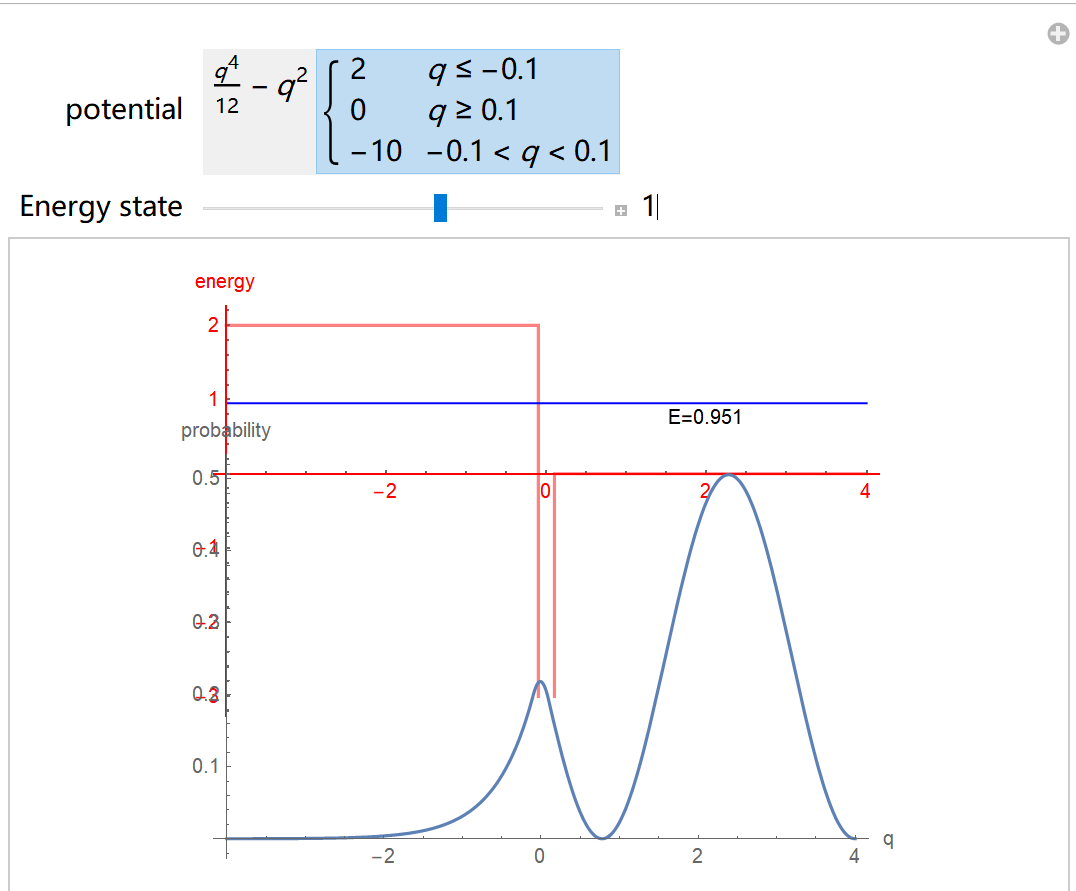
\includegraphics[scale=0.2]{P1.png}
        \caption{The first state eigenenergy for $a=0.1$}
    \end{figure}
    \begin{figure}[H]
        \centering
        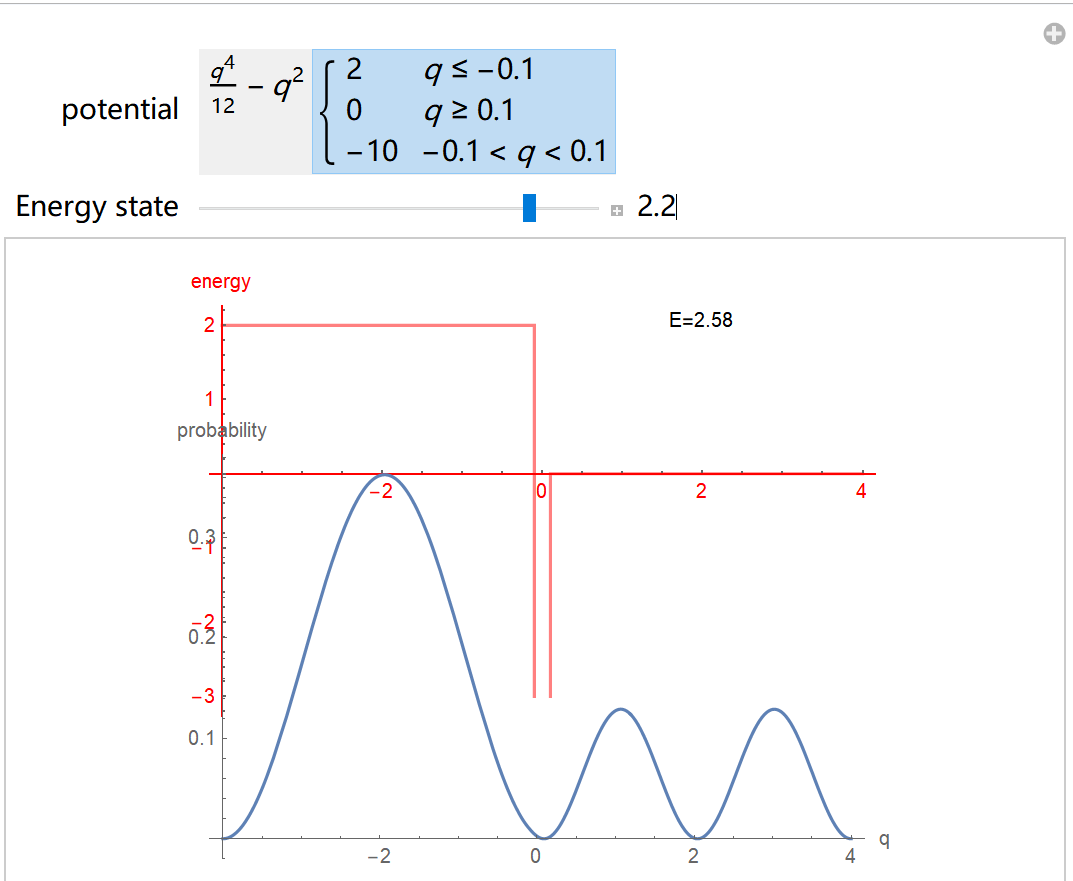
\includegraphics[scale=0.2]{P2.png}
        \caption{The second state eigenenergy for $a=0.1$}
    \end{figure}
\section{Problem 2}
    \begin{figure}[H]
        \centering
        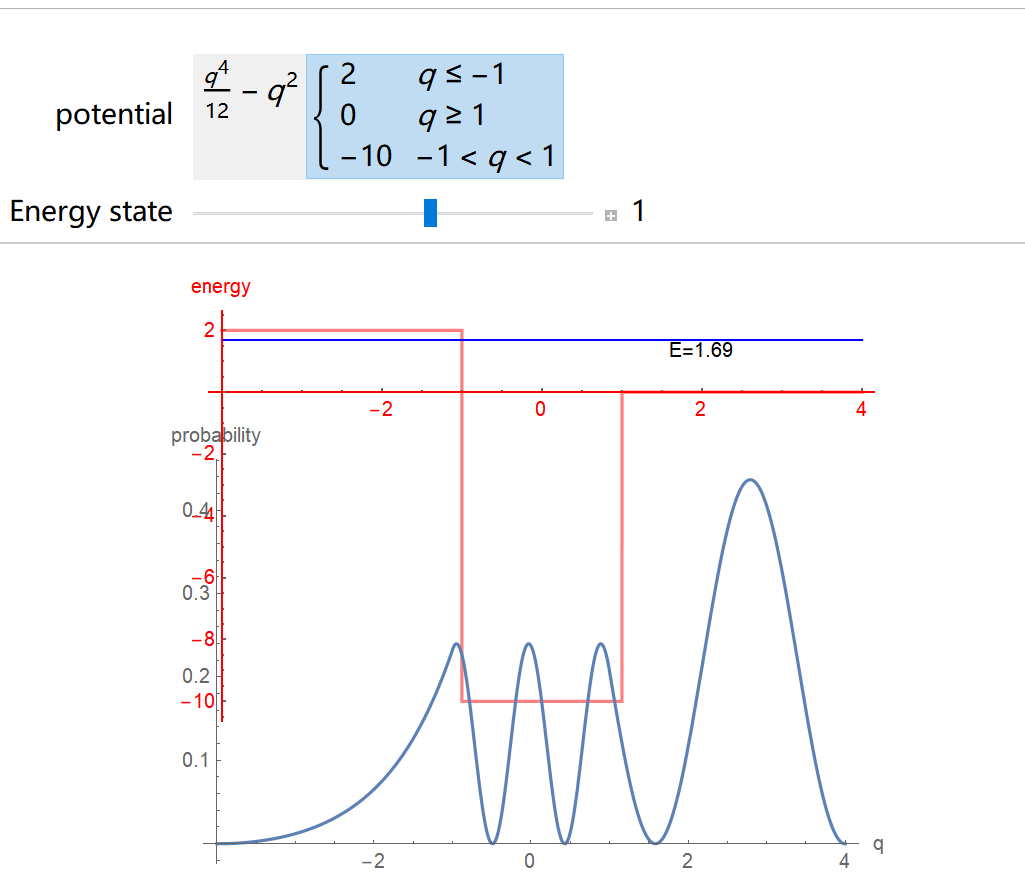
\includegraphics[scale=0.2]{P3.png}
        \caption{The first state eigenenergy for $a=1$}
    \end{figure}
    \begin{figure}[H]
        \centering
        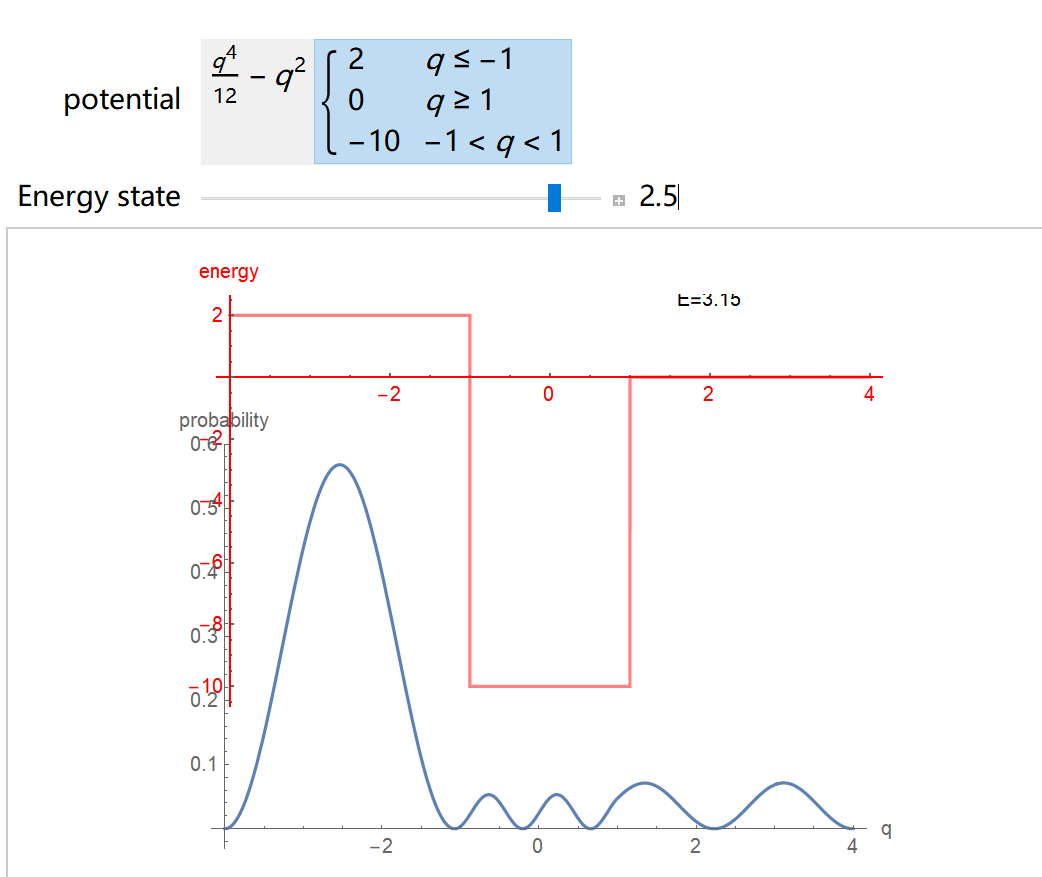
\includegraphics[scale=0.3]{P4.png}
        \caption{The second state eigenenergy for $a=2$}
    \end{figure}
    \begin{thebibliography}{99}
        \bibitem{1}https://demonstrations.wolfram.com/QuantumWellExplorer/
    \end{thebibliography}
\section*{Modified Mathematica Code}
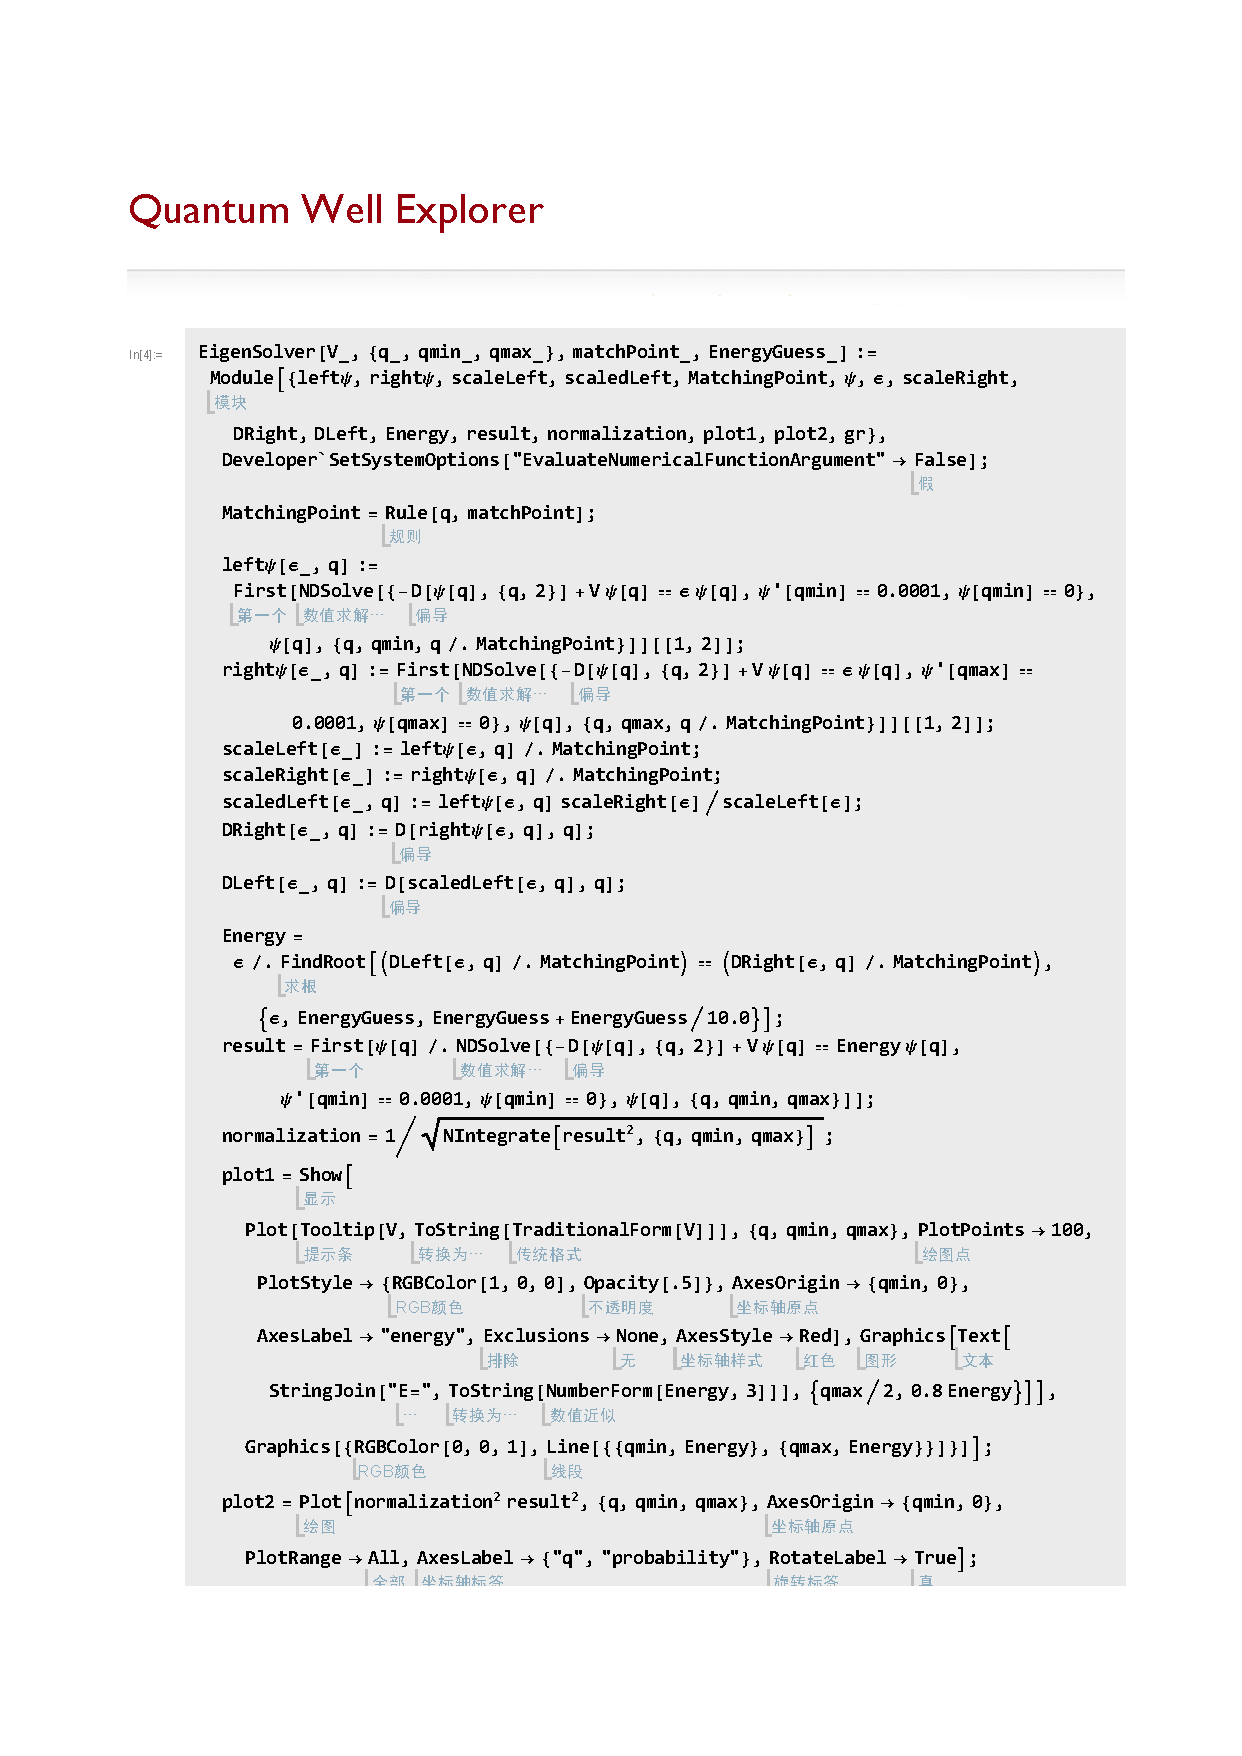
\includepdf[pages={1,2,3}]{Code.pdf}
\end{document}
